\documentclass[twoside]{report}
\usepackage[italian]{babel}
\usepackage[utf8]{inputenc}
\usepackage{amsmath}
\usepackage{amsthm}
\usepackage{amsfonts}
\usepackage{amssymb}
\usepackage{cancel}
\usepackage[margin=1in]{geometry}
\usepackage{hyperref}
\usepackage{bookmark}
\usepackage{setspace}
\usepackage{titlesec}
\usepackage{fancyhdr}
\usepackage{adjustbox}
\usepackage{float}
\usepackage{graphicx}

\graphicspath{{./images/}}

\setlength{\parskip}{0pt}
\titlespacing*{\subparagraph}{1em}{0em}{0em} 

\makeatletter
\renewenvironment{abstract}{%
    \if@twocolumn
        \section*{\abstractname}%
    \else
        \begin{center}%
            {\bfseries \abstractname\vspace{-.5em}\vspace{\z@}}%
        \end{center}%
        \small
        \begin{quotation}
    \fi}
    {\if@twocolumn\else\end{quotation}\fi}
\makeatother

\hypersetup{
    pdfauthor={Luca Facchini},
    pdftitle={Appunti di Sistemi Informativi},
    pdfsubject={Appunti del corso di Sistemi Informativi, tenuto dal prof. Bouquet Paolo presso l'Università degli Studi di Trento. Corso seguito nell'anno accademico 2024/2025.},
    pdfkeywords={Sistemi Informativi, Università degli Studi di Trento, Paolo Bouquet},
    pdfproducer={LaTeX},
    pdfcreator={pdflatex},
}

\fancypagestyle{chapterInit}{%
    \fancyhf{}
    \renewcommand{\headrulewidth}{0pt}
    \fancyfoot{}
    \fancyfoot[LE,RO]{\thepage}
    \fancyfoot[LO,RE]{"Appunti di Sistemi Informativi" di Luca Facchini}
}
\fancypagestyle{stdPage}{
    \fancyhead{}
    \fancyhead[RO,LE]{\leftmark}
    \setlength{\headheight}{15pt}
    \fancyfoot{}
    \fancyfoot[LE,RO]{\thepage}
    \fancyfoot[LO,RE]{"Appunti di Sistemi Informativi" di Luca Facchini}
}



\title{Appunti di Sistemi Informativi}
\author{Luca Facchini (mat. 245965)}
\date{A.A. 2024/2025}

\begin{document}
    \begin{titlepage}
        \centering  % Center everything on the title page
        {\Huge\textbf{Appunti di Sistemi Informativi}} \\[1cm] % Title
        \vspace{0.5cm}
        
        {\Large Luca Facchini} \\ % Author name
        \vspace{0.3cm}
        {\large Matricola: 245965} \\[2cm] % Additional author info
        
        {\large Corso tenuto dal prof. Casari Paolo} \\[0.3cm] % Course information
        {\large Università degli Studi di Trento} \\[1.5cm]
        
        {\large A.A. 2024/2025} \\[3cm] % Academic year
        
        % Abstract section with spacing control
        \vfill
        \begin{abstract}
            Questo documento contiene gli appunti del corso di Sistemi Informativi, tenuto dal prof. Casari Paolo presso l'Università degli Studi di Trento. Il corso è stato seguito nell'anno accademico 2024/2025.
        \end{abstract}
        
        \vfill  % Pushes the content to the center vertically
    \end{titlepage}

    \pagestyle{fancy}
    \fancyhead{}
    \fancyhead[RO,LE]{\leftmark}
    \setlength{\headheight}{15pt}
    \fancyfoot{}
    \fancyfoot[LE,RO]{\thepage}
    \fancyfoot[LO,RE]{"Appunti di Sistemi Informativi" di Luca Facchini}
    
    \begingroup
        \tableofcontents
        \thispagestyle{stdPage}
    \endgroup
    
    \include{chapters/01-laSocietàDellaConoscenza}
    
    \chapter{Concetti Generali sull'Informatica Aziendale}
\thispagestyle{chapterInit}
\section{Introduzione e definizioni}
    \paragraph{Informatica Aziendale} L'\textbf{informatica aziendale} è la disciplina che studia l'applicazione dell'informatica nelle aziende, studia inoltre l'influenza di questa nelle diverse categorie di un sistema aziendale. Esistono diversi settori di applicazione trai quali:
        \begin{itemize}
            \item \textbf{Aiuto e guida operativa} - Assistenza agli operatori a seguire le corrette procedure di lavoro con un costante controllo iterativo sui dati. Facilitazione di ricerca e recupero di informazioni.
            \item \textbf{Organizzativa} - Automazione di processi da un lato, richiesta di \textbf{competenze} e \textbf{risorse} differenti dall'altro.
            \item \textbf{Controllo} - Rilevazione di caratteristiche e comportamenti di un sistema, possibilità di \textbf{analisi quantitative} e \textbf{qualitative}.
            \item \textbf{Strategia} - Supporto ai processi di trasformazione e innovazione, supporto alle decisioni strategiche. 
        \end{itemize}
    \paragraph{Sistemi Informativi aziendali} I \textbf{sistemi informativi aziendali} sono l'insieme delle procedure e delle infrastrutture che definiscono e supportano l'elaborazione, la distribuzione e l'utilizzo delle informazioni all'interno di una azienda. Molto spesso ci si basa su una infrastruttura elettronica. È importante non confondere i sistemi informativi con i sistemi informatici, infatti è vero che ogni sistema informatico è un sistema informativo, ma non è vero il contrario.
    \paragraph{Risorse e processi}
        \subparagraph{Risorsa } Una \textbf{risorsa} "è tutto ciò con cui l'organizzazione opera" sia che questo possa essere un bene fisico o che questo sia un bene immateriale
        \subparagraph{Processo } Un \textbf{processo} è un insieme di attività atte a gestire una risorsa nel suo ciclo di vita.
\section{Sistema informativo aziendale}
    \paragraph{Definizione} Un \textbf{sistema informativo aziendale} è un sistema che permette di raccogliere, elaborare, memorizzare e distribuire informazioni all'interno di un'organizzazione. Questo sistema si compone di:
    \begin{itemize}
        \item \textbf{Dati}: \begin{itemize}
            \item di Configurazione - Dati che descrivono la struttura dell'organizzazione
            \item operativi - Dati che descrivono le attività dell'organizzazione
            \item di supporto - Dati che supportano le attività dell'organizzazione
            \item di stato - Dati che descrivono lo stato dell'organizzazione
        \end{itemize}
        \item \textbf{Procedure}: \begin{itemize}
            \item acquisizione - Raccolta di dati
            \item controllo ed elaborazione - Controllo e manipolazione dei dati
            \item pianificazione
        \end{itemize}
        \item \textbf{Mezzi e strumenti}: \begin{itemize}
            \item Hardware - sever e periferiche
            \item Stazioni di lavoro
            \item \dots
        \end{itemize}
    \end{itemize}
\section{Impatto dell'informatica nelle azienda}
    \subsection{Questioni da rispettare} 
        Il sistema \textbf{informatico} aziendale deve rispettare alcuni criteri per essere considerato adeguato:
        \begin{description}
            \item[Livello di astrazione] Il sistema deve essere in grado di rappresentare la realtà aziendale in modo corretto, sintetico ma completo.
            \item[Tempestività] Il sistema deve essere in grado di fornire le informazioni in tempo utile ed appropriato al contesto dell'operazione e della mole di dati.
            \item[Livello di copertura] Il sistema deve essere in grado di coprire tutte le aree aziendali e tutti i processi aziendali nei vari livelli di dettaglio.
        \end{description}
        Allo stesso tempo il sistema informativo deve \textbf{garantire}: Accessibilità dei dati e Correttezza del flusso, flusso che si divide in:
        \begin{description}
            \item[Orizzontale] tra le varie aree aziendali
            \item[Verticale] tra i vari livelli gerarchici
        \end{description}
    \subsection{Processi classi di un sistema informativo}
        Esistono tre classici processi informatizzati comuni a tutte le aziende che adottano un sistema informativo informatico:
        \begin{description}
            \item[Sviluppo funzioni operative] - Processo che si occupa di automatizzare dei processi che sono già presenti andando a ridurre i tempi e la mano d'opera necessaria.
            \item[Pianificazione] - Processo che prende i dati inseriti nel \texttt{SI} e li elabora per automatizzare processi di pianificazione.
            \item[Controllo] - Processo che renda automatico il controllo dei dati i inseriti nel \texttt{SI} e li confronta con criteri e dati di riferimento segnalando eventuali anomalie.
        \end{description}
    \label{subsec:nuoviProcessi}
    \subsection{Nuovi processi}
        \paragraph{Introduzione dell'informatica} L'introduzione dell'informatica in azienda non si occupa semplicemente di supporto a processi già esistenti, ma col tempo si aprono nuovi processi, innovativi, che prima non erano possibili.
        \paragraph{BRP} Nasce da questa idea il concetto di \textbf{Business Process Re-engineering} o \textbf{Reingegnerizzazione dei processi aziendali} che consiste nel ripensare e ridisegnare i processi aziendali per sfruttare al meglio le nuove tecnologie informatiche. La spinta verso il processo è generata dalla vasta adozione delle reti informatiche.
        \paragraph{Contatto col cliente al tempo di internet} Con l'avvento di internet e delle reti informatiche, il contatto con il cliente assume delle modalità completamente nuove, si passa da un contatto diretto a un contatto mediato da un sistema informatico, che per certi versi può essere più efficiente e più efficace.
\section{I sistemi informativi nelle aziende Italiane}
    \paragraph{Le aziende in italia} Le aziende in Italia assumono una conformazione molto differente rispetto al panorama europeo, infatti il 99,9\% delle aziende italiane sono \textbf{PMI} (Piccole e Medie Imprese) e solo lo 0,1\% sono grandi aziende.
    \paragraph{PMI e \texttt{SI}} Le PMI sono aziende che hanno una struttura molto semplice e che spesso l'investire in un sistema informativo non è una priorità visto che i processi sono molto semplici e non richiedono un sistema informativo complesso. \newline
    Spesso quindi un \texttt{SI} potrebbe essere visto come un costo inutile, ma con l'avvento di internet e delle nuove tecnologie, anche le PMI stanno iniziando ad adottare un sistema informativo in piccola misura, ovviamente non adotteranno \texttt{SI} di grandi dimensioni, ma sistemi informativi, spesso italiani in quanto più vicini alla realtà delle PMI, più piccoli e adeguati alle loro esigenze.


    \chapter[Struttura aziendale e del suo \texttt{SI}]{La struttura dell’azienda e del suo sistema informativo}
\thispagestyle{chapterInit}
\section{Concetto di esigenza informativa}
    \paragraph{Funzione \texttt{SI}} La funzione primaria del \textbf{sistema informativo} è quella di aiutare e guidare chi svolge mansioni che mandano avanti l'azienda attraverso queste. Inoltre il \texttt{SI} deve essere di aiuto e guida in modo diverso per aree diverse, ciò tramite il \textbf{livello d'astrazione} che sale man mano che si sale di livello gerarchico. L'\textbf{esigenza informativa} dipende dal tipo di attività svolta e dal livello gerarchico dell'utente. (es. i livelli operativi hanno bisogno di informazioni attuali ed precise spesso il singolo dato, mentre i livelli direzionali hanno bisogno di informazioni sintetizzate anche su periodi più lunghi).
    \subsection{Schema di Anthony}
        \paragraph{Schema di Anthony} L'organizzazione aziendale è vista a forma piramidale con i livelli operativi alla base, i livelli intermedi al centro e i livelli direzionali in cima. Ogni livello ha bisogno di informazioni diverse e quindi il \texttt{SI} deve essere in grado di fornire informazioni adeguate a ciascun livello.
        \begin{figure}[H]
            \centering
            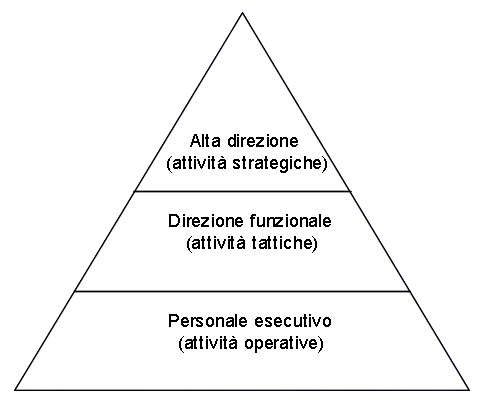
\includegraphics[scale = 0.5]{03/schemaAnthony.png}
            \caption{Schema di Anthony}
        \end{figure}\newpage
        \paragraph{profili informativi} Di seguito è riportata una tabella con i profili informativi di ciascun livello, si può notare come i livelli operativi abbiano bisogno di poche informazioni ma molto dettagliate, precise e in modo continuo, il livello direzionale tattico ha accesso ai dati con frequenza minore ma prefissata e con un livello di dettaglio minore produce quindi un volume medio di informazioni, il livello strategico ha bisogno di informazioni molto sintetizzate e con una frequenza molto bassa se non sporadica ma ha bisogno anche di informazioni esterne all'azienda.
        \begin{table}[H]
            \begin{adjustbox}{width=\textwidth}
                \begin{tabular}{|c|c|c|c|c|}
                    \hline
                    & \textbf{Frequenza} & \textbf{Dati} & \textbf{Provenienza dati} & \textbf{Volume} \\
                    \hline
                    \textbf{Livello direzionale strategico} & Sporadica & molto sintetizzati & interni ed esterni & basso \\
                    \hline
                    \textbf{Livello direzionale tattico} & Prefissata & sintetici e analitici & interni & medio \\
                    \hline
                    \textbf{Livello operativo} & Continua & analitici & interni & elevati \\
                    \hline
                \end{tabular}
            \end{adjustbox}
        \end{table}
\section{Sistemi operazionali}
    \paragraph{funzioni principali}
        \begin{itemize}
            \item Automazione di attività procedurali - In questo caso il \texttt{SI} è un supporto all'operatore
            \item Definizione di nuovi processi - come visto \hyperref[subsec:nuoviProcessi]{sottosezione 2.3.3}
            \item Aiuto nelle attività aziendali 
            \item Raccolta di dati - gli operatori inseriscono i dati nel sistema in modo continuo
            \item Guida per l'operatore - il sistema guida l'operatore nelle attività da svolgere in questo modo si riducono gli errori
        \end{itemize}
    \paragraph{Azioni sui dati}
        \begin{itemize}
            \item Accesso interattivo in inserimento, lettura, modifica - l'operatore può interagire con il sistema e modificare i dati nei limiti imposti 
            \item Trattamento di dati - il sistema tratta i dati in modo automatico e li presenta all'operatore in modo chiaro 
            \item Descrizione di eventi - il sistema descrive le transazioni e le attività svolte in modo da poterle ripetere in caso di necessità
            \item Valutazione e trattamento di informazioni utili - il sistema valuta i dati se sussistono errori e li segnala all'operatore
            \item Aggregazione per il calcolo di indicatori di stato - il sistema aggrega i dati per calcolare indicatori di stato dell'azienda
        \end{itemize}
    \paragraph{Componenti fondamentali}
        \begin{itemize}
            \item Base si dati operazionale - contiene i dati operativi dell'azienda
            \item Funzioni operative - funzioni che permettono di svolgere le attività operative
        \end{itemize}
\section{Sistemi informazionali}
    \paragraph{funzioni principali}
        \begin{itemize}
            \item Facilitazione del processo decisionale
            \item Presentazione dei dati secondo diverse aggregazioni e viste
            \item Confronto tra indicatori aziendali e indicatori esterni
        \end{itemize}
    \paragraph{Azioni sui dati}
        \begin{itemize}
            \item Accesso in lettura
            \item Aggregazione dei dati
            \item Descrizione di aree/temi
            \item Profondità temporale
            \item Multi-dimensionalità
        \end{itemize}
    \paragraph{Componenti fondamentali}
        \begin{itemize}
            \item Base dati informativa
            \item Strumenti di analisi
            \item Procedure di alimentazione (dati)
        \end{itemize}
\end{document}